\documentclass{article}

% Set page size and margins
% Replace `letterpaper' with `a4paper' for UK/EU standard size
\usepackage[letterpaper,top=2cm,bottom=2cm,left=3cm,right=3cm,marginparwidth=1.75cm]{geometry}

% Useful packages

\usepackage{amsmath}
\usepackage{graphicx}
\usepackage{ctex}
\usepackage{float}
\usepackage{listings}
\usepackage[colorlinks=true, allcolors=blue]{hyperref}
\usepackage{xcolor}
\definecolor{dkgreen}{RGB}{1,50,32}
\definecolor{mauve}{rgb}{0.58,0,0.82}

\lstset{
  basicstyle=\small\ttfamily,
  basewidth=0.5em,
  numbers=left,                    
  numberstyle=\tiny\color{gray},
  stepnumber=1,                   
  numbersep=10pt,                  
  tabsize=2,                      
  breaklines=true,                
  breakatwhitespace=false,
  xleftmargin=2em,
  language=Python,                
  frame=single,	                 
  rulecolor=\color{black},        
  keywordstyle=\color{blue},      
  commentstyle=\color{dkgreen},   
  stringstyle=\color{mauve},      
}

\title{AI B: Assignment 1}
\author{12110613 任嘉熙}

\begin{document}
\maketitle

\section{MAE(L1)Loss}

\subsection{定义}
L1Loss又称绝对误差损失,在回归问题中较为常用,在回归问题中我们的目标是预测一个连续的数值输出,而不是像分类问题一样预测的是离散的类别。L1Loss通过计算预测值与实际值之间的绝对差值来衡量模型的性能。

对单个样本,L1Loss被定义为:
$$
L(y,\hat{y})=\sum_{i=1}^{n}|y_i-\hat{y_i}|
$$
其中,y是我们的target,$\hat{y}$是模型给出的预测值,n是目标值的维度,$y_i$和$\hat{y_i}$分别是目标值和预测值的第i个元素。

\subsection{可视化结果}
记录模型每个epoch下的trainingLoss,testingLoss,trainingAccuracy,testingAccuracy,并绘制散点图。
\begin{figure}[H]
    \centering
    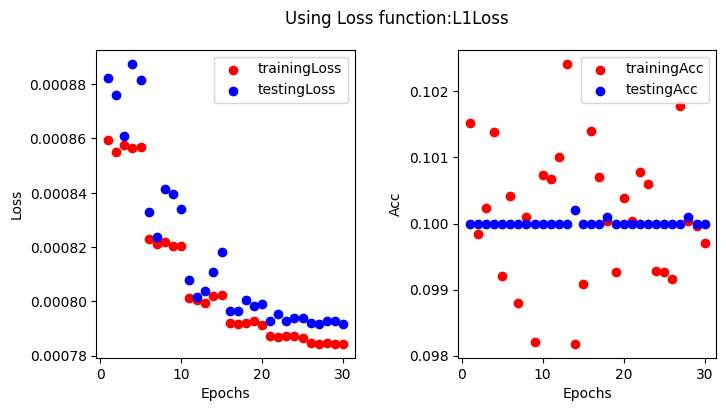
\includegraphics[width=0.9\textwidth]{Figure/L1Loss.png}
    \caption{L1Loss}
    \label{fig:L1Loss}
\end{figure}

\subsection{结果分析}
可以观察到,trainingloss和testingloss一直在下降,说明还没有出现过拟合现象,但是与此同时loss都很小且下降的幅度也很小。但可以从准确度观察到,在训练集的准确度呈波动状,表现得非常不稳定,而在测试集上表现为基本稳定在0.1,且这个模型是对输入预测为了十类,而准确度为0.1则表示分类分类的准确度为从十类中任意挑选了一类作为预测结果,模型并没有得到训练。

\section{CELoss}

\subsection{定义}
CrossEntropyLoss交叉熵损失多用于多分类问题,用来判定实际的输出与期望的输出的接近程度。实际的输出是我们的模型预测出来的得分,期望的输出则是一个one-hot向量,表示真实的标签(正确类别的索引是1,其余全是零)。

对单个样本,CrossEntropyLoss被定义为:
$$
L(y,\hat{y})=-\sum_{i}y_i · log(\hat{y_i})
$$
其中,y是我们期望输出的one-hot向量,$\hat{y_i}$表示模型预测的结果转换成的概率分布。

\subsection{可视化结果}

记录模型每个epoch下的trainingLoss,testingLoss,trainingAccuracy,testingAccuracy,并绘制散点图。
\begin{figure}[H]
    \centering
    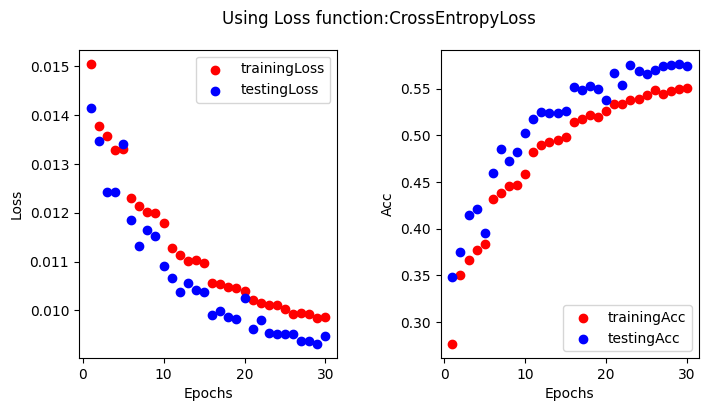
\includegraphics[width=0.9\textwidth]{Figure/CrossEntropyLoss.png}
    \caption{CrossEntropyLoss}
    \label{fig:CrossEntropyLoss}
\end{figure}

\subsection{结果分析}
可以观察到,trainingloss和testingloss随着epoch的增多呈下降趋势,且下降趋势减慢,呈收敛状,说明模型还没有出现过拟合的现象。且从准确度的角度来看,训练集和测试集上的准确度都呈上升状态,且上升的速度越来越慢,说明模型有收敛的趋势,且还没有达到过拟合,准确率能达到0.5左右,说明模型的泛化能力不错,模型已经有了一定的判断分类的能力。从总体来看,在测试集上的表现总要比训练集好,可能训练集和测试集的划分不理想,表现为测试集比训练集简单。

\section{FocalLoss}

\subsection{定义}
FocalLoss焦点损失是解决类别不平衡问题的损失函数,在目标检测和图像分割任务中表现良好,在许多机器学习的任务中类别分布通常是不均衡的,即某些类别的样本数量远远大于其他类别,这样会导致模型倾向于预测出现频率较高的类别而忽略了出现频率较低的类别。FocalLoss的目的是调整损失函数的权重,使模型更加关注难以分类的样本。

对单个样本,FocalLoss被定义为:
$$
FL(p_t)=-(1-p_t)^\gamma·log(p_t)
$$
其中,$p_t$是模型预测的类别概率,$\gamma$是一个用户定义的调节因子,通常取正数,用于调整难易样本权重。当增大$\gamma$,使相应的$(1-p_t)^\gamma$项增大,损失增加,模型会更加关注难以分类的样本。

\subsection{可视化结果}

记录模型每个epoch下的trainingLoss,testingLoss,trainingAccuracy,testingAccuracy,并分别绘制了在gamma=0.5和gamma=2的情况下的散点图。
\begin{figure}[H]
    \centering
    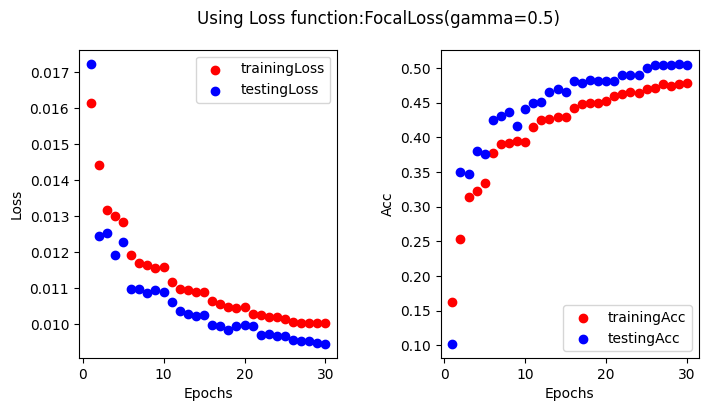
\includegraphics[width=0.9\textwidth]{Figure/FocalLoss(gamma=0.5).png}
    \caption{FocalLoss(gamma=0.5)}
    \label{fig:FocalLoss(gamma=0.5)}
\end{figure}

\begin{figure}[H]
    \centering
    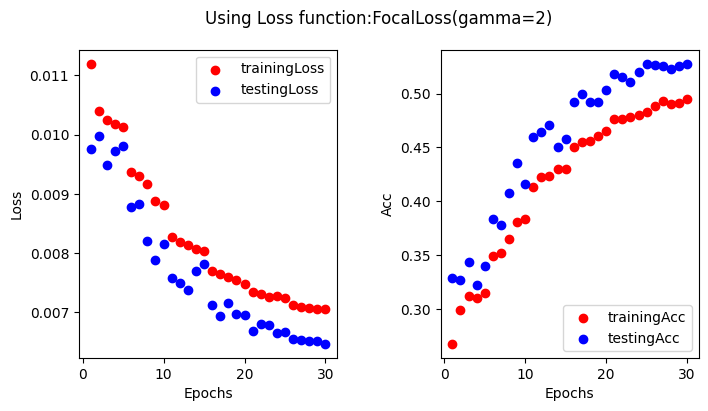
\includegraphics[width=0.9\textwidth]{Figure/FocalLoss(gamma=2).png}
    \caption{FocalLoss(gamma=2)}
    \label{fig:FocalLoss(gamma=2)}
\end{figure}

\subsection{结果分析}
可以观察到,当gamma取不同值时trainingloss和testingloss都随着epoch的增加而下降,且下降速度减缓,有收敛的趋势,说明在这期间还没有出现过拟合现象。在gamma=0.5时trainingloss和testingloss都比gamma=2的情况大,说明改变gamma的值对模型的训练还是有一定影响的,存在一部分难以分类的样本。从准确率的角度来看,在gamma=0.5和gamma=2的情况下都在呈上升趋势,且上升速率越来越慢,在gamma=2时准确率相较gamma=0.5时高一点,说明模型存在一定难分类的样本,且增加权重能让模型表现得更好。准确率均能达到0.5以上,说明模型的泛化能力不错。从整体上,模型在测试集表现得比测试集要好,应关注数据集的分布以及训练集和测试集的划分。

\section{比较分析}
我们将从几个不同的指标来对比这几个Loss function的表现,准确率(Accuracy)
、精准率(Precision)、召回率(Recall)和F1分数(F1 score)。通过横向对比几个损失函数分别在训练集和测试集上的表现,来观察他们的表现性能。
\subsection{准确率(Accuracy)}
准确率被定义为所有预测正确的样本的数量占样本总数的比例。实际上我们在以上可视化的结果中已经体现出来了,现把应用不同的损失函数时在相同批次下的准确率绘制在一张图上,便于我们更直观的观察其表现性能。
\begin{figure}[H]
    \centering
    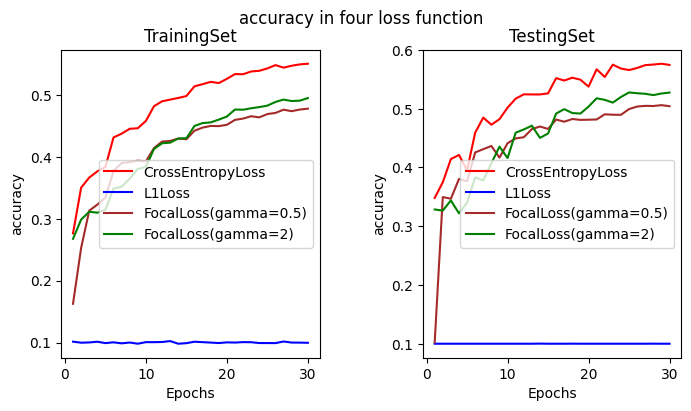
\includegraphics[width=0.8\textwidth]{Figure/Accuracy.png}
    \caption{Accuracy)}
    \label{fig:Accuracy}
\end{figure}
可以观察到,在训练集和测试集上都是CrossEntropyLoss函数表现得最好,当gamma=0.5时的FocalLoss函数与gamma=2时的FocalLoss函数接近,L1Loss函数表现得最差。在测试集上,准确率一直呈上升趋势,都没有明显的下降点,说明都没有出现过拟合现象。在分为十类的分类问题上准确率达到了接近0.6,说明模型在整体上表现得很好,泛化能力不错。

\subsection{精确率(Precision)}
精确率被定义为分类器预测为Positive的正确样本数量占所有预测为Positive的样本数量比例,精确率越高,说明模型在预测正类时出错的越少。在多分类任务中,需要分别计算每个类别的这样的比例,再进行加权平均得到最终的精确率结果。现把应用不同损失函数时在相同批次下的精确率绘制在一张图上,便于我们横向对比他们的表现性能。
\begin{figure}[H]
    \centering
    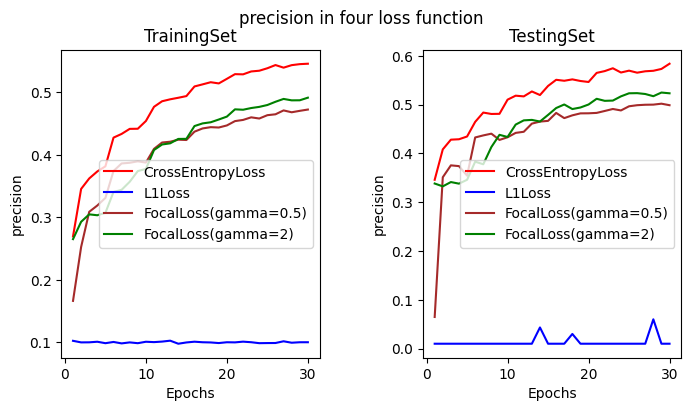
\includegraphics[width=0.8\textwidth]{Figure/Precision.png}
    \caption{Precision}
    \label{fig:Precision}
\end{figure}
可以观察到相似的结论,在训练集和测试集上都是CrossEntropyLoss的精确率表现得最好,当gamma=0.5时的FocalLoss函数和当gamma=2时的FocalLoss函数表现接近,L1Loss函数在训练集上较稳定地差,表现为随机分类,在测试集上虽然在批次增大时有一定波动,但是相较其他几个损失函数表现都差多了,甚至在差的时候精确度达到了接近0的水平。最终表现为在测试集上有接近0.6的精确率,模型在每一类上的预测都表现得不错。

\subsection{召回率(Recall)}
召回率被定义为分类器预测为Positive的正确样本数量占所有实际为Positive的样本数量的比例,召回率月高,说明模型找到正类样本的能力越强。在多分类任务中,召回率采用的计算方式与精确率类似。现把应用不同损失函数时在相同批次下的召回率绘制在同一张图上,便于我们横向观察他们的表现性能。
\begin{figure}[H]
    \centering
    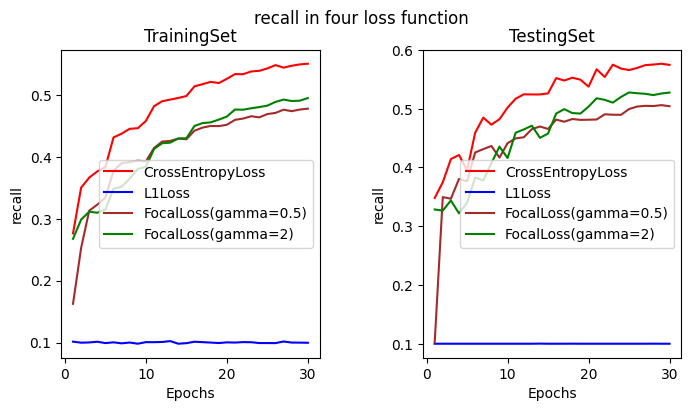
\includegraphics[width=0.9\textwidth]{Figure/Recall.png}
    \caption{Recall}
    \label{fig:Recall}
\end{figure}
通过对数值进行观察,发现我们计算出的召回率和准确率一模一样。对数据集进行观察,发现这是一个平衡的数据集,表现为在这个数据集中每种类别的数量完全相等。所以从召回率我们得到的结论应与准确率一致,即CrossEntropyLoss函数表现得最好,能达到接近0.6的召回率,说明对于每种类别,模型能找到这个类别的大部分正类样本。

\subsection{F1分数(F1 Score)}
F1分数被定义为精确率和召回率的调和平均数,他试图在这两个指标之间找到一个平均。如果F1分数很高,则说明我们的模型在精确率和召回率之间达到了一个好的平衡,兼顾二者,这往往是实践上比较重要的一个指标。现把应用不同损失函数时在相同批次下的F1分数绘制在同一张图上,便于我们进行相互对比。
\begin{figure}[H]
    \centering
    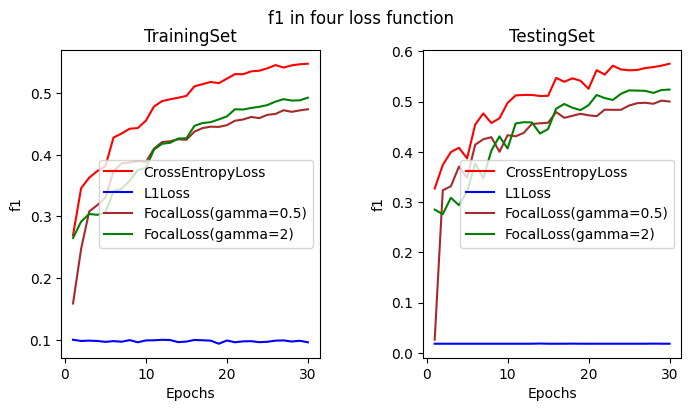
\includegraphics[width=0.9\textwidth]{Figure/F1Score.png}
    \caption{F1Score}
    \label{fig:F1Score}
\end{figure}
可以观察得到,我们仍然得到在应用CrossEntropyLoss时的表现最好,FocalLoss(gamma=0.5)和FocalLoss(gamma=2)的表现接近,L1Loss的表现远低于其他三个函数。说明CrossEntropyLoss函数较好的平衡了模型在精确率和召回率的表现,兼顾了在预测中误判和漏判的两种情况,且在避免这两种情况的方面上表现得都不错。最终也能达到接近0.6的水平。

\section{总结}
\subsection{结论分析}
综合从各个指标考虑,CrossEntropyLoss函数表现得最好,FocalLoss(gamma=0.5)和FocalLoss(gamma=2)的表现接近,L1Loss函数表现得远差于其他损失函数。

从定义上看,L1Loss并不适合于做分类任务,它计算的是预测值与真实值之间的差距,且分类问题中的值都是离散的,关心的是能否正确预测出样本的类别,用这样的损失很难衡量分类器的准确性,使模型很难进行学习。且我们使用的优化器是随机梯度下降(SGD),L1Loss在零点处不可导,在较小的损失值处也有着较大的梯度,难以收敛。

而FocalLoss(gamma=0.5)和FocalLoss(gamma=2)在这个数据集上表现得也不错,且在数据集是完全平衡的条件下,通过观察数据集,可能是因为在这个数据集中存在相似的类别,使得分类器难以辨别,通过FocalLoss提高对难以分类的样本的权重,来提高模型对这些类别的关注度 ,提高模型的表现性能。且增加模型对这类样本的关注度能提升这个损失函数的表现性能。但我们能观测到,增加的表现能力并不多,可能我们也不宜过大关注这类样本,可能会造成过拟合现象,说明这类样本在数据集中的确存在,但数量并不多。

CrossEntropyLoss函数是分类任务的常用选择,测量的是模型输出的概率分布与真实标签的概率分布之间的差异。通过最小化负对数似然,来最大化模型对真实标签的预测概率。且我们采用的是SGD操作,CrossEntropy对于这个优化器是相对友好的,提供了梯度信息,帮助模型快速并准确调整参数。且在数值计算上比其他的损失函数更稳定,通过对数函数减少了数值上的不稳定性。

\subsection{实现分析}
通过查阅,在Pytorch中并没有FocalLoss函数的实现,于是基于这里只关注gamma的变化,定义了一个简单的FocalLoss类:
\begin{lstlisting}
class FocalLoss(nn.Module):
    def __init__(self, gamma=2, alpha=None):
        super(FocalLoss, self).__init__()
        self.gamma = gamma
        self.alpha = alpha

    def forward(self, inputs, targets):
        # 计算交叉熵损失
        ce_loss = F.cross_entropy(inputs, targets, reduction='none', weight=self.alpha)
        # 计算焦点损失
        pt = torch.exp(-ce_loss)
        focal_loss = ((1 - pt) ** self.gamma) * ce_loss
        return focal_loss.mean()
\end{lstlisting}

为了减小误差,数据集的训练是shuffle的,如果每次重新运行整段代码会很麻烦,且会因为每次的训练集可能不一样造成误差。于是我们采用同一次数据集训练,使用同一个模型,在每次训练完后会清除训练痕迹,且重新定义优化器以清除优化器上面的参数痕迹,再更换另一个损失函数:
\begin{lstlisting}
def reset_model(model):
    for layer in model.children():
     if hasattr(layer, 'reset_parameters'):
            layer.reset_parameters()
\end{lstlisting}

将训练过程包装成方法,以train batch,test batch,损失函数为输入参数,在每次训练结束再去清除痕迹便于下一次采用其他损失函数训练:
\begin{lstlisting}
def modeltraining(func1,func2,criterion):
    optimizer = optim.SGD(model.parameters(), lr=LEARNING_RATE, momentum=MOMENTUM)
    scheduler = torch.optim.lr_scheduler.StepLR(optimizer, step_size=STEP,gamma=GAMMA)
    ...
    reset_model(model)
    return training_loss,training_acc,testing_loss,testing_acc,training_precision,training_recall,training_f1,testing_precision,testing_recall,testing_f1
\end{lstlisting}

由于CrossEntropyLoss函数会自动调用Softmax函数,且接收的input参数是模型的原始输出数据,而其他三种方法都需要我们对模型输出的向量进行一定处理,于是采用包装函数,便于我们更改模型所采用的损失函数:
\begin{lstlisting}
def wrapper(func):
    def new_func(model,image,target,criterion):
        target=F.one_hot(target,num_classes=10).float()
        return func(model,image,target,criterion)
    return new_func
\end{lstlisting}

最后我们在训练过程的函数中将各种用于评估的指标作为数组返回出来,便于我们后续画图分析。

\subsection{不足与可改进的地方}
\begin{itemize}
    \item 从几项指标来看,模型的表现还没有完全收敛,可以适当继续增加epoch的数量以提升模型的表现。
    \item 这个数据集是平衡的,在某些指标上表现一致。可以用其他的数据集来尝试是否会让模型的表现更好。
    \item 可以尝试更换优化器与更换优化器的超参,观察是否会影响模型的表现。在更换超参时也要相应地对模型的参数进行更改。
    \item 基于任务的需要定义更多的评估指标,例如灵敏度等。在这些已分析的指标都是分类任务重常见的指标。
\end{itemize}

\end{document}